%pdflatex abra.tex
%convert -density 150x150 abra.pdf abra.png
\documentclass[border={2pt 2pt 2pt 2pt}]{standalone}
\usepackage{tikz}
\usetikzlibrary{calc}
\begin{document}

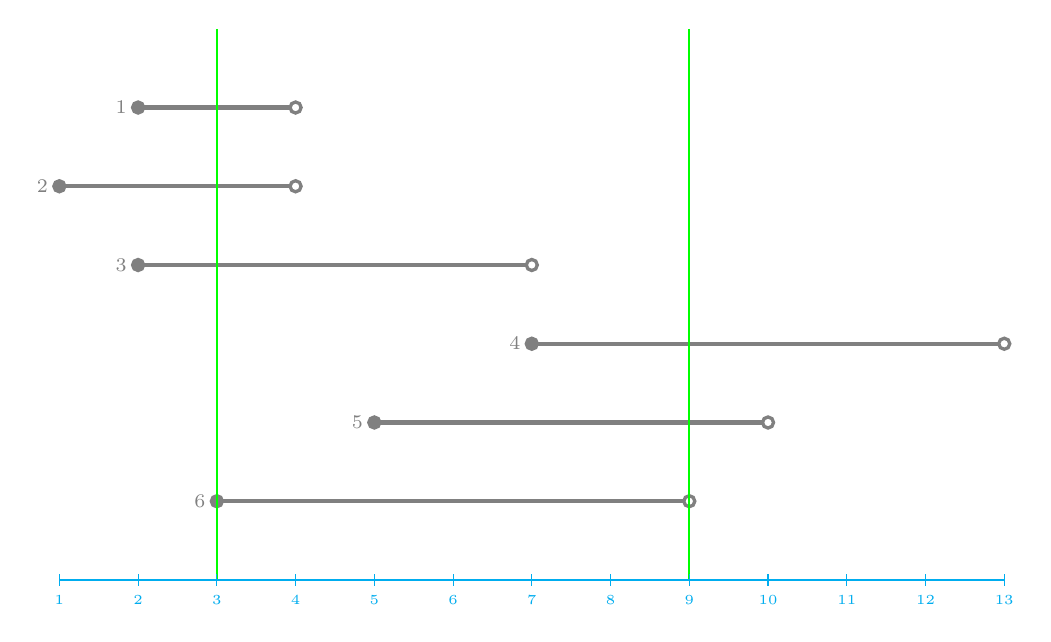
\begin{tikzpicture}[scale=1]
\coordinate (A1) at (2,0);
\coordinate (A2) at (4,0);
\coordinate (B1) at (1,-1);
\coordinate (B2) at (4,-1);
\coordinate (C1) at (2,-2);
\coordinate (C2) at (7,-2);
\coordinate (D1) at (7,-3);
\coordinate (D2) at (13,-3);
\coordinate (E1) at (5,-4);
\coordinate (E2) at (10,-4);
\coordinate (F1) at (3,-5);
\coordinate (F2) at (9,-5);
\draw[gray,ultra thick] (A1)node[left]{\scriptsize 1}--(A2);
\draw[gray,ultra thick] (B1)node[left]{\scriptsize 2}--(B2);
\draw[gray,ultra thick] (C1)node[left]{\scriptsize 3}--(C2);
\draw[gray,ultra thick] (D1)node[left]{\scriptsize 4}--(D2);
\draw[gray,ultra thick] (E1)node[left]{\scriptsize 5}--(E2);
\draw[gray,ultra thick] (F1)node[left]{\scriptsize 6}--(F2);
\draw[gray,very thick,fill=gray] (A1) circle [radius=0.07];
\draw[gray,very thick,fill=white] (A2) circle [radius=0.07];
\draw[gray,very thick,fill=gray] (B1) circle [radius=0.07];
\draw[gray,very thick,fill=white] (B2) circle [radius=0.07];
\draw[gray,very thick,fill=gray] (C1) circle [radius=0.07];
\draw[gray,very thick,fill=white] (C2) circle [radius=0.07];
\draw[gray,very thick,fill=gray] (D1) circle [radius=0.07];
\draw[gray,very thick,fill=white] (D2) circle [radius=0.07];
\draw[gray,very thick,fill=gray] (E1) circle [radius=0.07];
\draw[gray,very thick,fill=white] (E2) circle [radius=0.07];
\draw[gray,very thick,fill=gray] (F1) circle [radius=0.07];
\draw[gray,very thick,fill=white] (F2) circle [radius=0.07];
%\draw[blue,very thick,fill=white] (A) circle [radius=0.5];
%\node at (A) {\huge\bf 1};
\draw[green,thick] (3,1)--(3,-6);
\draw[green,thick] (9,1)--(9,-6);
\draw[cyan,thick](1,-6)--(13,-6);
\foreach \x in {1,...,13}
  \draw[cyan,xshift=\x cm] (0,{-6cm+2pt})--(0,{-6cm-2pt}) node[cyan,below,fill=white]{\tiny\x};
\end{tikzpicture}

\end{document}
